
%%%%%%%%% MASTER -- compiles the 4 sections

\documentclass[11pt,letterpaper]{article}

%%%%%%%%%%%%%%%%%%%%%%%%%%%%%%%%%%%%%%%%%%%%%%%%%%%%%%%%%%%%%%%%%%%%%%%%%
\pagestyle{plain}                                                      %%
%%%%%%%%%% EXACT 1in MARGINS %%%%%%%                                   %%
\setlength{\textwidth}{6.5in}     %%                                   %%
\setlength{\oddsidemargin}{0in}   %% (It is recommended that you       %%
\setlength{\evensidemargin}{0in}  %%  not change these parameters,     %%
\setlength{\textheight}{8.5in}    %%  at the risk of having your       %%
\setlength{\topmargin}{0in}       %%  proposal dismissed on the basis  %%
\setlength{\headheight}{0in}      %%  of incorrect formatting!!!)      %%
\setlength{\headsep}{0in}         %%                                   %%
\setlength{\footskip}{.5in}       %%                                   %%
%%%%%%%%%%%%%%%%%%%%%%%%%%%%%%%%%%%%                                   %%
\newcommand{\required}[1]{\section*{\hfil #1\hfil}}                    %%
\renewcommand{\refname}{\hfil References Cited\hfil}                   %%
\bibliographystyle{abbrvnat}                                              %%
%%%%%%%%%%%%%%%%%%%%%%%%%%%%%%%%%%%%%%%%%%%%%%%%%%%%%%%%%%%%%%%%%%%%%%%%%

%PUT YOUR MACROS HERE
\usepackage{change page} % for indentation of sections
\usepackage{lipsum}
\usepackage{hyperref} %for urls
\usepackage{graphicx} %for includegraphics
\usepackage[table]{xcolor} %for table line color alteration
\usepackage{enumitem}  %fancy enumerated lists
\usepackage{wrapfig} %wrap text around figures
\usepackage[leftcaption]{sidecap} % side captions
\sidecaptionvpos{figure}{c} %position side caption

\usepackage[round,authoryear]{natbib} %biblio format!
\usepackage{multirow} %multirow tables
\usepackage{booktabs} %funky tabs in tables
\newcommand{\jri}[1]{\textcolor{blue}{ \emph{\scriptsize  #1}} }
\newcommand{\mbh}[1]{\textcolor{red}{ \emph{\scriptsize  #1}} }
\renewcommand{\thesubsection}{Objective \Roman{subsection}}
\renewcommand{\thesubsubsection}{\thesubsection\Alph{subsubsection}}
\renewcommand{\theenumi}{\Alph{enumi}}
\newcommand{\zp}{\emph{parviglumis}}
\newcommand{\zpp}{\emph{perennis}}
\newcommand{\zd}{\emph{diploperennis}}
\newcommand{\zl}{\emph{luxurians}}
\newcommand{\zm}{\emph{mexicana}}
\newcommand{\zh}{\emph{huehuetenangensis}}

%\includeonly{NSFsumm}

\begin{document}
%%%%%%%%%%%%% Project Summary max 1 page must include Intellectual Merit and Broader Impact) %%%%%%%%%%%%%%%%%%%
\setcounter{page}{1}

%%%%%%%%% PROJECT SUMMARY -- 1 page, third person
% e.g:  "The PI will prove" not "I will prove"

%Below are the pagination, font size, spacing and margin
%instructions for NSF proposals: \\
%
%FastLane does not automatically paginate a proposal.
%Each section of the proposal must be individually
%paginated prior to upload to the system. \\
%
%Use Computer Modern family of fonts at a font size of 11 points or
%larger. A font size of less than 10 points may be used for mathematical
%formulas or equations, figure, table or diagram captions and when
%using a Symbol font to insert Greek letters or special characters.
%The text must still be readable. The use of small type not in compliance with the NSF guidelines
%may be grounds for NSF to return the proposal without review. \\
%
%No more than 6 lines of text within a vertical space of 1 inch. \\
%
%Margins, in all directions, must be at least an inch. \\
%
%
\required{Project Summary}

\paragraph{Overview} The proposed project will investigate the genome-wide effects of hybridization and introgression in the genus \emph{Zea}.  First, investigators will study  incipient speciation between the lowland-adapted \emph{Z. mays} ssp. \emph{parviglumis} (hereafter, \emph{parviglumis}) and the highland-adapted \emph{Z. mays} ssp. \emph{mexicana} (hereafter, \emph{mexicana}).  Through field collections, genotyping and common garden studies, the investigators will assess what fraction of the genome is porous to gene flow in hybrid zones, how fitness of these taxa varies across a hybrid zone, and how allele frequency clines are patterned at adaptive loci. Second, investigators will determine the impact of hybridization and introgression between domesticated maize (\emph{Z. mays} ssp. \emph{mays}) and wild  \emph{Zea}. Population genomic analyses of sympatric collections will be used to assess whether maize served as a bridge for gene flow between otherwise allopatric \emph{Zea} species and whether maize received gene flow from wild relatives that facilitated its adaptation to new environments.

% This should be a brief statement of the problem you plan to address.
% It should look something like an abstract. 

%The project summary should be a description of the proposed activity suitable
%for publication, no more than one page in length. It should not be
%an abstract of the proposal, but rather a self-contained description of
%the activity that would result if the proposal were funded. The summary
%should be written in the third person and include a statement of objectives
%and methods to be employed. It should be informative to other persons
%working in the same or related fields and understandable to a scientifically
%or technically literate lay reader. \\
%
%The summary must clearly address in separate statements (within the one-page summary):
%the intellectual merit of the proposed activity; and the broader impacts
%resulting from the proposed activity. Proposals that do not separately
%address both criteria within the one-page Project Summary will be returned without
%review. \\

\paragraph{Intellectual Merit}  Much progress has been made in the study of hybridization and introgression through the development of theory, through field-based ecological research, and through genetic analyses based on a limited number of molecular markers. However, much remains to be discovered regarding how these evolutionary processes have shaped genomes. The research proposed here will leverage the genomic resources of the maize model system to investigate how hybridization and introgression have molded the genomes of both wild \emph{Zea} species and domesticated maize on two different timescales: 1) An evolutionary timescale covering 60,000 generations of divergence between \emph{parviglumis} and \emph{mexicana}; and 2) An ecological timescale in which maize has spread across the Americas and adapted to local conditions. The analysis on an evolutionary timescale will generate basic knowledge on the process of incipient speciation and the porous nature of the genomes of diverging species, whereas the analysis on an ecological timescale can inform, for example, the study of biological invasions and the role of introgression in facilitating rapid local adaptation.

% This is why your project is interesting and will help further
% knowledge in the field of mathematics. 

%How important is the proposed activity to advancing
%knowledge and understanding within its own field or across different fields?
%How well qualified is the proposer (individual or team) to conduct the project?
%(If appropriate, the reviewer will comment on the quality of prior work.)
%To what extent does the proposed activity suggest and explore creative, original,
%or potentially transformative concepts? How well conceived and organized is the
%proposed activity? Is there sufficient access to resources?  \\

\paragraph{Broader Impacts}

The investigators will achieve societally relevant outcomes in the proposed project by providing STEM training opportunities for undergraduate and graduate students, participating in Iowa State University�s GK12 Fellowship program, and establishing an exchange program between universities in the United States and Mexico. This project will provide ample training opportunities for both undergraduate and graduate students in laboratory, computational, and field-based research. The investigators have successfully recruited minority students into their research programs in the past and will make every effort to do so as part of this proposed work. The graduate student funded to work at Iowa State University will participate in the University's GK12 program that serves the Des Moines public school system. Through this opportunity, the graduate student will bring their research on maize evolution into the classrooms of the most diverse public school system in the state of Iowa. The \emph{Zea} study system provides an excellent opportunity to deliver evolution training to middle and high school students in a state dominated by maize agriculture. Finally, the proposed exchange program would create an opportunity for students from the United States to conduct research internationally and allow these students to interact with visiting students from Mexico. Through these interactions, students will be better prepared for modern STEM research, which is often highly collaborative and international in nature.

% There are 4 kinds of broader impacts.
% 1. advance discovery and understanding while promoting teaching,
% training and learning
% 2. broaden the participation of underrepresented groups
% 3. disseminated broadly to enhance scientific and technological
% understanding
% 4. benefits of the proposed activity to society

% Max 1 page
%%%%%%%%%%%%%
 Project Description max 15 pages (usually) Must include discussion of recent Prior (last 5 years) %%%%%%%%%%%%%%%%%%%
\setcounter{page}{1}
%%%%%%%%% PROJECT DESCRIPTION  -- 15 pages (including Prior NSF Support)

\required{Project Description}
\begin{center}
%\emph{Maximum of 15 pages}
\end{center}
%The Project Description (including Results from Prior NSF Support, which is
%limited to five pages) may not exceed 15 pages. Visual materials, including charts,
%graphs, maps, photographs and other pictorial presentations are included in the
%15-page limitation. PIs be cautioned that the project description must
%be self-contained and that URLs that provide information related to the proposal
%should not be used. \\
%
%All proposals to NSF are reviewed utilizing the two merit review criteria,
%intellectual merit and broader impacts. \\
%
% The Project Description should provide a clear statement of the work 
% to be undertaken and must include: objectives for the period of the proposed 
% work and expected significance; relation to longer-term goals of the PI's 
% project; and relation to the present state of knowledge in the field, 
% to work in progress by the PI under other support and to work in progress 
% elsewhere.

%%%%%%%%%%%%%%%%%%%%%%%%%%%%%%%%%%%%%%%%%%%%%%%%%%%%%%%%%%%%%%%%%%%%%%
%INTRO
%%%%%%%%%%%%%%%%%%%%%%%%%%%%%%%%%%%%%%%%%%%%%%%%%%%%%%%%%%%%%%%%%%%%%%
\section*{Introduction}

While the potential roles of hybridization and introgression as agents of evolution have long been appreciated \citep{Anderson1948, Anderson1954, Stebbins1959}, only recently have technological innovations allowed for characterization on a genome-wide scale. Multiple genome-wide studies have now reported substantial inter-taxon introgression in both plant \citep{Hufford2013, renaut2013} and animal \citep{consortiumbutterfly2012, staubach2012} species. Introgression has been found across substantial portions of genomes and specifically at loci thought to underlie adaptation. 

In the investigation proposed here, we will build upon our previous work in maize (\emph{Zea mays} ssp. \emph{mays}) and its wild relatives (\emph{Zea} spp.; collectively referred to as teosinte) in order to characterize the evolutionary role of hybridization and introgression in the genus \emph{Zea}. This study system is ideally suited for such research due to its well-characterized history, large natural populations, and the availability of exceptional genomic resources \citep{Hufford2012}. The history of \emph{Zea} allows us to assess the genome-wide effects of hybridization and introgression at two different timescales: 1) A more evolutionary timescale spanning 60,000 generations of divergence amidst gene flow between the subspecies \emph{Zea mays} ssp. \emph{parviglumis} and \emph{Zea mays} ssp. \emph{mexicana}; and 2) An ecological timescale ($\sim$3000-9,000 generations) in which maize has spread across the Americas and adapted to local conditions, potentially through hybridization and introgression from endemic wild relatives that are allopatric to the progenitor of maize. Our analysis on an evolutionary timescale will generate basic knowledge of the process of incipient speciation and the porous nature of genomes of diverging species, whereas our analysis on an ecological timescale can inform, for example, the study of biological invasions if maize is viewed as an invasive species aided in colonization by gene flow from locally-adapted native species.

%%%%%%%%%%%%%%%%%%%%%%%%%%%%%%%%%%%%%%%%%%%%%%%%%%%%%%%%%%%%%%%%%%%%%%
%OBJECTIVES
%%%%%%%%%%%%%%%%%%%%%%%%%%%%%%%%%%%%%%%%%%%%%%%%%%%%%%%%%%%%%%%%%%%%%%
\section*{Objectives}
	
We will leverage the resources of the \emph{Zea} study system to address two primary objectives:

\subsection*{Objective I: Hybrid Zones: Assess the evolutionary significance of hybridization and introgression in locally-adapted, parapatric wild \emph{Zea} taxa}
\emph{Zea mays} ssp. \emph{parviglumis} (the wild progenitor of maize; hereafter, \emph{parviglumis}) and \emph{Zea mays} ssp. \emph{mexicana} (hereafter, \emph{mexicana}) diverged approximately 60,000 BP \citep{Ross-Ibarra2009a} and have parapatric distributions: while \emph{parviglumis} occurs in the warm lowlands of southwest Mexico, \emph{mexicana} is found in the cool highlands of the Mexican Central Plateau. Narrow regions of substantial admixture between these wild subspecies have been discovered at middle elevations \citep{Fukunaga2005, Pyhajarvi2013}. Through targeted collections, generation of high-density genotyping data, population genomic analyses, and common garden experiments, we will address the following research questions and work toward establishing this system as a model for the study of hybrid zones:
\begin{adjustwidth}{5em}{5em}
\subsubsection*{\emph{Research Question IA) What fraction of the genome is porous to gene flow in hybrid zones?}}

\subsubsection*{\emph{Research Question IB) How does the fitness of \emph{parviglumis}, \emph{mexicana}, and hybrid populations vary across the hybrid zone?}}

\subsubsection*{\emph{Research Question IC) Are allele frequency clines at loci associated with fitness traits in \emph{mexicana} and \emph{parviglumis} steeper than those at non-associated loci?}}
\end{adjustwidth}
\vspace{0.5cm}

\subsection*{Objective II: Genus-wide Introgression: Determine the extent to which hybridization and introgression have altered the \emph{Zea} genus during the post domestication spread of maize}
Maize was domesticated in southwest Mexico from \emph{parviglumis} $\sim$9,000 BP \citep{Matsuoka2002} and quickly spread throughout North America, bringing this crop into sympatry with new species of teosinte \citep{Vigouroux2008a}. Through a combination of dense genotyping of range-wide samples of maize and teosinte and targeted, full-genome sequencing, we will assess three questions regarding the importance of introgression during the spread of maize:
\begin{adjustwidth}{5em}{5em}	
\subsubsection*{\emph{Research Question IIA) Was the spread of maize facilitated by gene flow from locally-adapted wild \emph{Zea}?}}
\subsubsection*{\emph{Research Question IIB) What is the geographic scale of adaptive introgression?}}
\subsubsection*{\emph{Research Question IIC) Did maize serve as a bridge for gene flow between previously isolated \emph{Zea} taxa?}}
\end{adjustwidth}
\vspace{0.5cm}

%%%%%%%%%%%%%%%%%%%%%%%%%%%%%%%%%%%%%%%%%%%%%%%%%%%%%%%%%%%%%%%%%%%%%%
%RATIONALE AND SIGNIFICANCE
%%%%%%%%%%%%%%%%%%%%%%%%%%%%%%%%%%%%%%%%%%%%%%%%%%%%%%%%%%%%%%%%%%%%%%
\section*{Rationale and Significance}
Pioneers in evolutionary biology including G. Ledyard Stebbins and Edgar Anderson recognized the important role hybridization and introgression could play in adaptation and speciation \citep{Anderson1948, Anderson1954}. These evolutionary forces were thought to be particularly influential when environmental conditions encountered by a species were marginal, variable, or new \citep{Stebbins1959}. More recently, theoretical and empirical investigations of hybridization have focused on hybrid zones, defined as regions where distinct taxa co-occur and mate, resulting in progeny of mixed ancestry \citep{HarrisonHybridZone}. 

While hybrid zone theory has progressed and many compelling empirical examples have been identified based on hybrid morphology and limited genetic data \citep{Delmore2013, Galindo2013, Parchman2013, Smith2013a}, several outstanding questions remain. Additional study is needed to determine whether hybrid zones are primarily maintained as tension zones in which hybrids are selected against or as ecotones where hybrids have an advantage under certain environmental conditions \citep{Kruuk1999, Rasmussen2012, Smith2013b}. Moreover, genome-wide analysis of the fraction of the genome that is porous to gene flow in hybrid zones is rare and will likely offer considerable insight.  For example, vanguard genomic studies of hybridization and introgression suggest that rates of gene flow vary substantially across loci and that chromosomal rearrangements (\emph{e.g.}, inversions and translocations) may restrict gene flow in hybridizing species \citep{Hufford2013, Barb2014, Poelstra2014, SoriaCarrasco2014}.
	 
Both wild and domesticated \emph{Zea} offer exciting opportunities to study hybridization. The subspecies \emph{parviglumis} and \emph{mexicana} are distributed across a steep altitudinal gradient and differ for traits that are thought to be adaptive in the highlands such as the presence of macrohairs and stem pigmentation.  Both of these traits are found in highland \emph{mexicana} but are lacking in lowland \emph{parviglumis}. Analysis of $\sim$100 microsatellite markers genotyped in a range-wide sample of \emph{parviglumis} and \emph{mexicana} has previously identified elevated admixture between the subspecies in two geographically-distinct, mid-elevation regions: eastern Jalisco state and the eastern Balsas River Basin \citep{Fukunaga2005}.  The positioning of these populations at intermediate locations between the known distributions of the two subspecies suggests they may represent stable zones of hybridization.

Our recent genome-wide analysis ($\sim$40,000 SNPs) of a population from the putative eastern Balsas hybrid zone revealed extensive subspecies admixture across all individuals sampled \citep{Pyhajarvi2013}.  Genotype data from this hybrid population were compared to those of non-admixed populations revealing relatively short shared haplotypes between these two groups, a result suggesting continual gene flow between \emph{parviglumis} and \emph{mexicana} at this hybrid zone over a substantial period of time \citep{Pyhajarvi2013}.  Longer shared haplotypes were found in the hybrid population in chromosomal regions identified as potential inversions based on high differentiation and linkage disequilibrium between \emph{parviglumis} and \emph{mexicana} \citep{Pyhajarvi2013}.  These regions may be particularly resistant to gene flow.  While these initial findings are suggestive of hybrid zone dynamics in teosinte, further population genomic investigation is necessary to compare the genomic architecture of hybridization and introgression both across populations within hybrid zones as well as between distinct hybrid zones.  Furthermore, evaluation of the fitness of \emph{parviglumis}, \emph{mexicana}, and hybrid samples in reciprocal transplants will shed light on whether hybridization of teosinte subspecies is sustained through tension zone or ecotone processes (see \textbf{Objective I}).

In addition to the ongoing hybridization between \emph{parviglumis} and \emph{mexicana} occurring since divergence $\sim$60,000 BP, gene flow between domesticated maize and various taxa of the genus \emph{Zea} has been detected based on both hybrid morphologies observed in the field \citep{wilkes1967teosinte, Wilkes1977} and genetic data \citep{Ross-Ibarra2009a}. Domestication of maize from \emph{parviglumis} occurred recently on an evolutionary timescale ($\sim$9,000BP; \citealt{Matsuoka2002}) and was followed by rapid spread of the crop across the Americas during the following millennia \citep{Piperno2001,Grobman2012}. During this diffusion maize was brought into sympatry with new wild relatives that were likely allopatric to the progenitor of maize (\emph{i.e., parviglumis}) for long periods prior to domestication \citep{hufford2012inferences}. 

Our recent work has provided evidence of introgression from \emph{mexicana} into maize during its earliest diffusions into the highlands of the Mexican Central Plateau.  Consistent introgression into maize was found in several highland maize populations at QTL for phenotypes (\emph{e.g.}, pigment and macrohairs) that distinguish highland \emph{mexicana} from lowland \emph{parviglumis} \citep{Hufford2013}. Our interpretation of this result is that maize received adaptive introgression from \emph{mexicana} that allowed the crop to spread into the highlands of Mexico. 

Subsequent to its diffusion into the Mexican highlands, maize spread into sympatry with additional teosinte taxa in Guatemala including \emph{Zea luxurians} (hereafter, \emph{luxurians}) and \emph{Zea mays} ssp. \emph{huehuetenangensis} (hereafter, \emph{huehuetenangensis}). Based on analysis of a small number of loci ($n=456$) \mbh{is this the number of SNPs in the 26 nuclear loci?}, \emph{mexicana} haplotypes have been found segregating in \emph{luxurians} \citep{Ross-Ibarra2009a}.  Since \emph{mexicana} and \emph{luxurians} are entirely allopatric in their distributions, this suggests maize has served as a bridge for gene flow between these two taxa.  Further work will be necessary to explore this possibility and to assess if maize has, more generally, altered the genomes of \emph{Zea} species through gene flow during its spread across the Americas.  Yet another fascinating question that remains to be answered is whether additional \emph{Zea} taxa, like \emph{mexicana}, have donated adaptive alleles to maize that allowed it to successfully colonize new habitats (see \textbf{Objective II}).

%%%%%%%%%%%%%%%%%%%%%%%%%%%%%%%%%%%%%%%%%%%%%%%%%%%%%%%%%%%%%%%%%%%%%%
%PRELIMINARY RESULTS
%%%%%%%%%%%%%%%%%%%%%%%%%%%%%%%%%%%%%%%%%%%%%%%%%%%%%%%%%%%%%%%%%%%%%%
\section*{Preliminary Results}

Our previous publications suggest \emph{Zea} is a promising model system for exploring the evolutionary role of hybridization and introgression (\emph{e.g.},  \citealt{Ross-Ibarra2009a, vanheerwaarden2011a, Hufford2013, Pyhajarvi2013}).  To further refine our research questions and provide preliminary results for this proposal we have analyzed a previously published data set \citep{vanheerwaarden2011a, Fang2012} of 983 SNPs genotyped across a panel of $>2,000$ samples including all subspecies and species of teosinte and an Americas-wide sample of maize landraces (\emph{i.e.}, ancient farmer varieties of maize).  While the low density of the markers in this data set precludes genome-wide inferences and haplotype-based analyses, the comprehensive taxon sampling makes this an ideal resource for guiding future research.

\subsection*{Evidence for hybrid zones between \emph{parviglumis} and \emph{mexicana}}

We have assessed evidence for admixture between \emph{parviglumis} and \emph{mexicana} using the range-wide sampling of hundreds of populations in the 983-SNP data set.  The probability of each sample's assignment to \emph{parviglumis} and \emph{mexicana} groups was calculated using the program STRUCTURE \citep{Pritchard2000} and individuals were sorted in order of increasing altitude.  We find that individuals from several mid-elevation populations show appreciable assignment to both \emph{parviglumis} and \emph{mexicana} groups (red underscored individuals in Figure \ref{fig:structure}) and likely represent hybrid populations.  

\begin{figure}
  \centering
   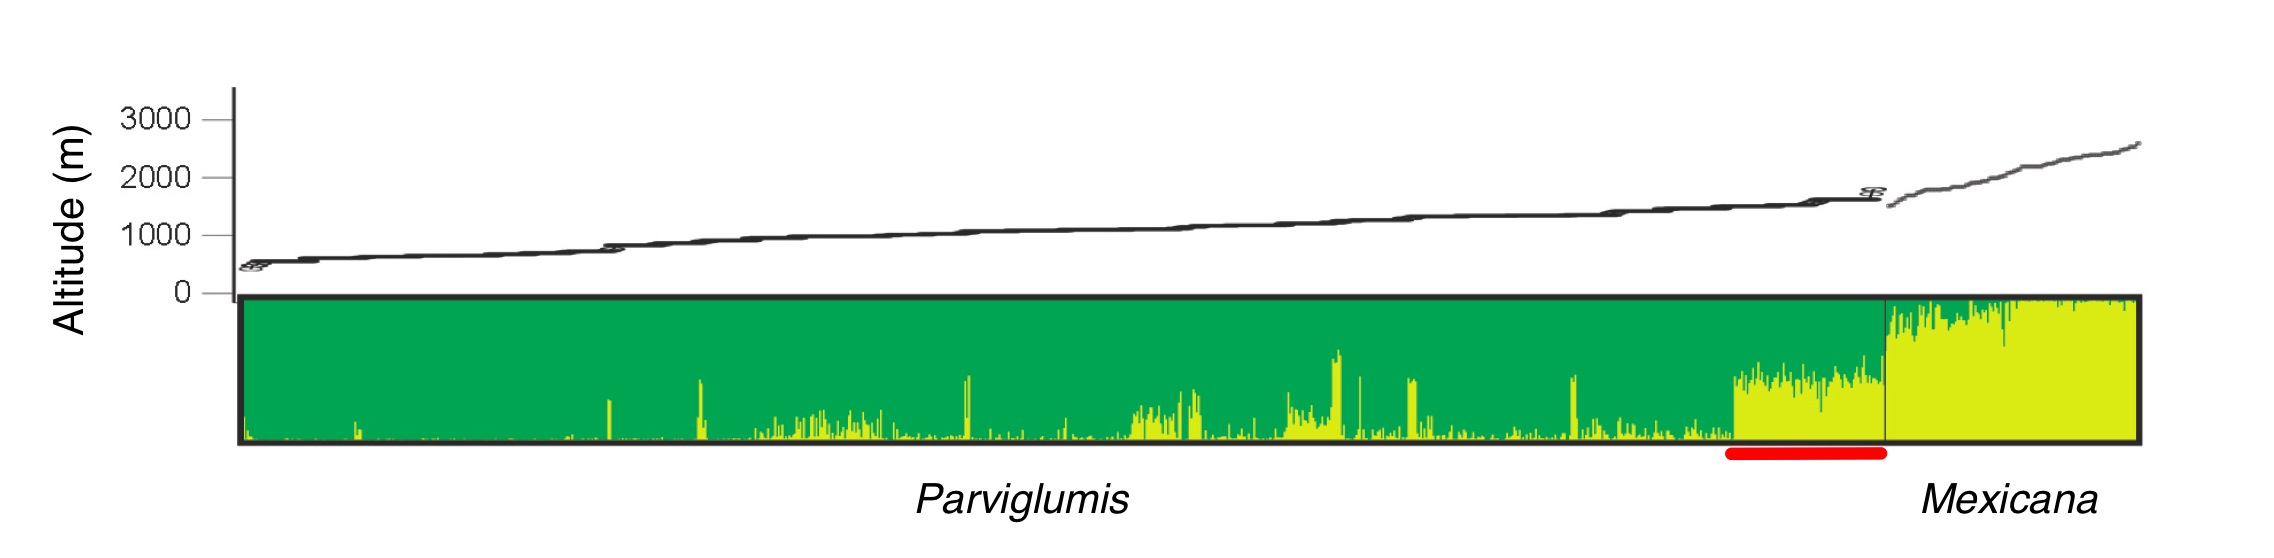
\includegraphics[width=0.95\textwidth]{structure.jpg}
    \caption{Assignment of \emph{parviglumis} and \emph{mexicana} individuals to K=2 groups using the Bayesian assignment algorithm of STRUCTURE \citep{Pritchard2000}.  Individuals are sorted by increasing altitude as indicated by the plot above the bar chart. Individuals from mid-elevation, hybrid zone populations are underscored in red.} 
\label{fig:structure}
\end{figure}

Several admixed populations cluster in two geographically distinct regions of Mexico: the eastern Balsas River Basin and eastern Jalisco state.  These locations fall at intermediate locations between the main distributions of \emph{parviglumis} and \emph{mexicana} (Panel A, Figure \ref{fig:pies}).  Hybrid populations from eastern Jalisco state are found at higher elevation (average elevation = 1632m) than hybrid populations in the eastern Balsas (average elevation = 1531m) and also show a higher proportion of membership in a \emph{mexicana} (\emph{i.e.}, highland teosinte) group (Panels B and C, Figure \ref{fig:pies}).  These findings suggest that hybrid populations from distinct environments may vary in proportion of ancestry from these two subspecies in a manner that is adaptive.  Estimates of pairwise population differentiation also suggest that hybrid populations in the Balsas and Jalisco are distinct in that Jalisco populations are less differentiated from \emph{mexicana} than hybrid populations in the Balsas (Table \ref{tab:Fst}).  Not surprisingly, populations in both hybrid zones are less differentiated from \emph{mexicana} and \emph{parviglumis} than these subspecies are from each other.

\begin{SCfigure}
  \centering
   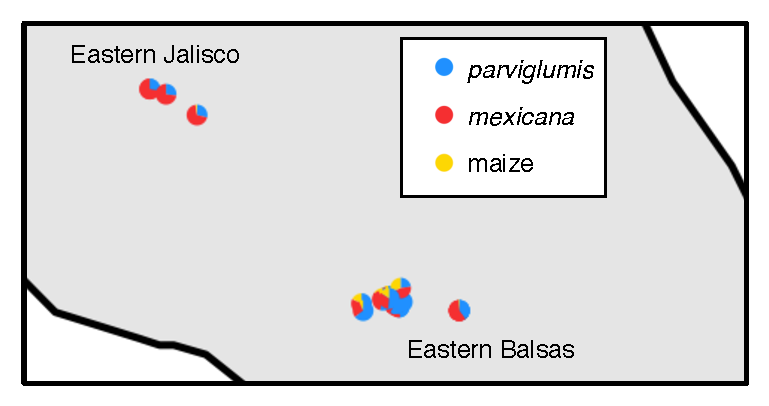
\includegraphics[width=0.6\textwidth]{pies.pdf}
    \caption{Proportion of assignment of hybrid populations to \emph{parviglumis}, \emph{mexicana}, and maize groups in putative Eastern Jalisco and Eastern Balsas hybrid zones} 
\label{fig:pies}
\end{SCfigure}

\begin{table}[]
\rowcolors{2}{gray!25}{white}
\begin{center}
\caption{Pairwise $F_{ST}$ between teosinte and hybrid populations} \label{tab:Fst}
\begin{tabular}{lcccc}\\\toprule
{\bf Taxon}&{\bf \emph{parviglumis}}&{\bf \emph{mexicana}}&{\bf Jalisco Hybrids}&{\bf Balsas Hybrids}\\\midrule
{\bf \emph{parviglumis}}&---&---&---&---\\
{\bf \emph{mexicana}}&0.107&---&---&---\\
{\bf Jalisco Hybrids}&0.059&0.064&---&---\\
{\bf Balsas Hybrids}&0.057&0.074&0.034&---\\\bottomrule
\end{tabular}
\end{center}
\end{table} 

\subsection*{Evidence for hybridization across the genus \emph{Zea}}

TreeMix Results\\

ILS Results\\

Chr4 Inversion Results?\\

%%%%%%%%%%%%%%%%%%%%%%%%%%%%%%%%%%%%%%%%%%%%%%%%%%%%%%%%%%%%%%%%%%%%%%
%SPECIFIC OBJECTIVES
%%%%%%%%%%%%%%%%%%%%%%%%%%%%%%%%%%%%%%%%%%%%%%%%%%%%%%%%%%%%%%%%%%%%%%
\section*{Research Plan}

\subsection*{Objective I: Hybrid Zones}

\subsubsection*{Research Question IA) What fraction of the genome is porous to gene flow in hybrid zones?}

Currently, very few studies have dissected the genome-wide architecture of hybridization and introgression in a hybrid zone (but see \citealt{staubach2012}). Genome-wide studies in teosinte are feasible at very high marker density \citep{Hufford2012b, Hufford2013, Pyhajarvi2013} and are also informed by the genomic resources of maize \citep{Hufford2012}, often providing detailed functional annotation for loci of interest, a rarity in other natural systems.  We will assess the genomic architecture of hybridization in two putative hybrid zones of \emph{mexicana} and {parviglumis} through careful collections and assembly of a study panel, generation of genome-wide marker data, and application of recently-developed population genomic analyses appropriate to this question.

\paragraph{\emph{Panel Construction and Sample Collection:}}
We currently have access to extensive collections of \emph{parviglumis}, \emph{mexicana}, and maize from throughout their respective ranges.  Moreover, Senior Personnel Luis Eguiarte and collaborator Salvador Montes-Hernandez (see attached letter of commitment) have recently collected altitudinal transects of \emph{parviglumis} and \emph{mexicana} that extend through both hybrid zones targeted by our project \citep{Diez2013} and are therefore familiar with populations in this region.  However, current collections will not be sufficient for both the genotyping and common garden activities we propose here and we have therefore budgeted for a collection trip during the first year of the project. We have already obtained the requisite collection permits as well as permits for importing samples into the United States for genetic analysis. Additionally, we have collaborations in place to facilitate co

\paragraph{\emph{Sample Genotyping:}}

\paragraph{\emph{Population Genomic Analyses:}}

\subsubsection*{Research Question IB) How do \emph{parviglumis}, \emph{mexicana}, and hybrid fitness vary across the hybrid zone?}

In order to assess whether \emph{Zea} hybrid zones exist through tension zone or ecotone dynamics we will conduct common garden experiments in Mexico at three altitudes: 1) Below a hybrid zone in regions occupied by \emph{parviglumis}; 2) Within a hybrid zone; and 3) Above a hybrid zone in regions occupied by \emph{mexicana}. Our experiments will gauge relative fitness between \emph{parviglumis}, \emph{mexicana}, and hybrids at each of these sites.
	
\subsubsection*{Research Question IC) Are allele frequency clines at loci associated with fitness traits in \emph{mexicana} and \emph{parviglumis} steeper than those at non-associated loci?}

We will combine our genome-wide marker data with data collected in our common garden experiments in order to perform genome-wide association analysis of fitness-related
phenotypes in \emph{parviglumis}, \emph{mexicana}, and hybrids. We will evaluate both the shape and slope of allele frequency clines at fitness-related loci relative to neutral loci.

II) Sample Genotyping: For sample genotyping we will utilize a reduced representation approach to next-generation sequencing called Genotyping By Sequencing (GBS) (Elshire et al. 2011). To date, this method has been used to genotype $>45,000$ maize samples and a bioinformatics pipeline (TASSLE-GBS) has been constructed that allows for genotyping at ~1,000,000 SNPs in maize (Glaubitz et al. In Press). The GBS methodology has been successfully applied to teosinte and is an ideal genotyping methodology for our proposed project due to the high marker density it provides in combination with a lack of ascertainment bias.

III) Population Genomic Analyses: For Objectives I and II, in addition to standard population genetic measures of differentiation and introgression (\emph{e.g.}, FST, shared and fixed variants between populations, Reich�s f statistics, patterns of linkage disequilibrium) we will implement recently-developed, haplotype-based methods for detecting hybridization and introgression (\emph{e.g.}, Price et al. 2009; Lawson 2012). Association analyses in Objective I will be carried out using the software package TASSEL. In Objective II, we will evaluate evidence for selection on introgressed loci using both haplotype- (\emph{e.g.}, Voight 2006) and frequency-spectrum- based (\emph{e.g.}, Nielsen et al. 2005) approaches as well as comparisons of environmental association (\emph{e.g.}, Coop et al. 2010). 

IV) Common Garden Experiments: Common garden experiments will be carried out at three field sites in Mexico: 1) At an altitude below a hybrid zone in regions occupied by \emph{parviglumis}; 2) Within a hybrid zone; and 3) At an altitude above a hybrid zone in regions occupied by \emph{mexicana}. We will collect fitness-related phenotypes in these experiments including percent germination, germination rate, plant height at 15-day intervals, seed set, seed weight, total-above-ground biomass, and survival.

\subsection*{Objective II: Genus-wide introgression}

\subsubsection*{Research Question IIA) Was the spread of maize facilitated by gene flow from locally-adapted wild \emph{Zea}?} 

*background on spread of maize

*one new habitat was highlands

* talk about Hufford 2013: Our recently published study of \emph{mexicana}/maize hybridization in sympatric populations (Hufford et al. 2013) suggests widespread adaptive introgression from \emph{mexicana} into maize. 

* but what about spread to (insert something about environment differences) in gautemala? 

* background on luxurians and huehue, information on maize arrival in guatemal from arch. record if available, or on maize in guat from van heerwaarden 2011.

* 4 pairs of huehue/maize and 4 pairs of lux/maize sympatric pops, then at both high and low elevation (or some other gradient?) we pick 1 allopatric teo and 1 allopatric maize, for a total of 6 pops of each taxa = 24 pops total.  

* 12 individuals per pop, GBS to 48 plex.

*D stats, g-statistic, pi <- no need for phasing

* phase with fastphase, run hapmix or other methods

* look for evidence of selection (Nielsen sweepfinder, etc.)

* can look for overlap with QTL for water-logging etc. traits (Mano papers) or GWAS for related traits in maize

* include formal analysis using Berg's SQuaT approach?

* additional questions: how much diversity remains in lux populations? what is connectivity of these pops? are lux and/or huehue threatened by introgression from maize? important to Guatemala as it is unique diversity to that country

We will also expand the scope of our previous work and assess whether similar patterns of introgression can be detected in maize populations that are sympatric to the Guatemalan teosintes (\emph{huehuetenangensis} and \emph{luxurians}).

\subsubsection*{Research Question IIB) What is the geographic scale of adaptive introgression?}

* in many plants local adaptation exists on a very fine geographical scale (examples, citations)

* previous work suggested introgression from mexicana allowed maize to adapt to highlands, and most of the introgression was ancient, suggesting adaptation to a broad set of challenges associated with higher elevations

* but we did see differences among populations (cite examples)

* now with increase resolution we can look at individual sympatric population pairs
<<<<<<< HEAD

* revisit introgression, show evidence of selection w/in individual pops
=======
* we also know parv hybridizes with maize, but unclear if any of the sympatric introgression is adaptive
* 3 pairs of mex/maize sympatric pops
* 3 pairs of parv/maize sympatric pops
* introgression, search for evidence of selection w/in individual pops
>>>>>>> 1961c83b07c16d726ba9f1c326041ce089abf480

\subsubsection*{Research Question IIC) Did maize serve as a bridge for gene flow between previously isolated Zea taxa?}

Our previous work based on a small number of loci has suggested that maize served as a bridge between \emph{parviglumis/mexicana} and \emph{huehuetenangensis} and \emph{luxurians} which are otherwise allopatric (Ross-Ibarra et al. 2009). The high-density, genome-wide data generated here will provide an opportunity to test the hypothesis that introgression occurred indirectly between previously allopatric \emph{Zea} taxa via maize as a conduit for gene flow.

* Inv4m appears in luxurians, but Tanja says is derived in mexicana

* JRI 2009 shows evidence of mex/lux gene flow

* other taxa (Wilkes thesis) like diploperennis, though these are more geographically restricted

* we will GBS 2 pops of each diplo and perennis to look for evidence of maize introgression. we do not have access to sympatric pops

* evaluate evidence for haplotype sharing among these. look for long haplotypes, G stats, etc.

* ask whether those coincide with regions that show evidence of introgression from maize.  

\section*{Broader Impacts}

Our efforts to broaden the impact of the research proposed here will begin within our groups through our commitment to effectively mentor volunteer undergraduate interns as well as graduate students and/or postdoctoral scholars funded by the project. Students and postdocs will receive one-on-one training from the investigators and senior personnel on laboratory, computational, and field research methods.  Mentees will also be encouraged and funded to present their work at scientific conferences.  Our groups have an excellent mentoring track record with four undergraduate students in the last five years publishing their work in scholarly journals and multiple underrepresented minorities participating in our research.

\subsection*{ISU GK12 Fellowship Program}
	
In addition to the student and postdoc mentoring that will occur within our groups, as part of our broader impact activities one of our graduate students will participate in Iowa State University's GK12 Fellowship program. The selected graduate student will spend one full day each week in a science middle or high school classroom for the entire academic year in the Des Moines Public School District. This is the largest and most diverse school district in Iowa. The graduate student will introduce the K12 students to the scientific process through inquiry-based activities, relate the students� science curriculum to real world examples, work with students on their science fair projects, and serve as a role model in a STEM profession. Furthermore, the graduate student will introduce students to his/her research project on hybridization and introgression in \emph{Zea}, a topic that is particularly well suited for teaching evolution in Iowa given the important role that maize plays in the Iowan economy. In introducing his/her dissertation research, the graduate student will engage Des Moines students in how research is conducted and provide STEM content professional training to his/her partner teacher. 

\subsection*{US-Mexico Exchange Program}
	
Finally, we will establish a student exchange program between the Eguiarte Laboratory at UNAM in Mexico and the Hufford and Ross-Ibarra Laboratories in the United States. The Ross-Ibarra Laboratory has run an NSF-supported, US-Mexico exchange program for the last three years.  All of the exchange students involved in the program have continued on to additional graduate work, and two have earned authorship on forthcoming papers from their internship.  We will build upon the success of this program.  A student from the Eguiarte group will spend 2-3 months in either the Hufford or Ross-Ibarra Laboratory learning the GBS methodology and/or honing his/her skills in population genomic analysis, whereas a student from the Hufford and/or Ross-Ibarra Laboratories will travel to Mexico to participate in sample collection trips and to obtain expertise in common garden field experiments. This exchange will build capacity in all groups involved and will provide a valuable international research experience for a graduate student supported by the grant.  

Senior Personnel Claudia Calderon has previously led international student research trips and will assist in preparing students from both the United States and Mexico for the exchange program. A survey will be given to both exchange students and faculty in order to gauge expectations prior to the trip and facilitate collaborations amongst the labs.  The survey will also assess students' knowledge and preconceived ideas  regarding their travel destinations.  A meeting (online or face-to-face) with the cohort of students traveling will help address these pre-conceptions and reduce cultural misunderstandings.  Suggestions will be given to students of how to prepare before the trip (visa, immigration requirements) and how to communicate with their peers and others during their exchange.  Students will be given information regarding the facilities where they will be staying, transportation to be used, food and water safety, the availability of telecommunications and general safety guidelines. \jri{be forewarned that exchange is a lot of work -- finding housing, taking care of visas, etc.  also may be tricky paying a student from Mexico who is at UCDavis.} \mbh{yep, we're limiting this to two interns (one to the US and one to Mexico) during years two and three.  Hopefully this will be manageable}

\required{Results From Prior NSF Support}
% 5 pages or fewer of the 15 pages for entire description document.
% include results from NSF grants received in the past 5 years.
% If supported by more than one grant, choose the most relevant one.

% For each grant, include: 
%	(a) NSF award number, amount, dates of support 
%	(b) The title of this project
%	(c) Publications resulting from this research
%	(d) Summary of the results of the completed work
%	(e) A brief description of data samples available and other research products not described 	      elsewhere
%	(f) For renewed support, a description of the relationship between the completed and 			      proposed work

% Due to space limitations, it is often advisable to use citations rather
% than putting the titles of the publications in the body 
% of this section

\subsection*{Ross-Ibarra: \#1238014: Biology of Rare Alleles in Maize and Its Wild Relatives}
\$13,311,185 (\$2,368,767 to Ross-Ibarra and \$1,206,211 to Flint-Garcia), 05/15/13-04/30/18. PI Edward Buckler, co-PIs J. Doebley, J. Holland, S. Flint-Garcia, Q. Sun, P. Bradbury, S. Mitchell, J. Ross-Ibarra
\par\noindent{\bf Intellectual merit} In the first year we have developed accurate imputation approaches, found evidence for the importance of deleterious variants and non-genic polymorphisms in heterosis and GWAS, documented differences in recombination among the parents of the NAM population, and found population genetic evidence suggesting the importance of demography and purifying selection across the genome.  The grant has produced 18 total publications in its first year (only publications involving PIs Flint-Garcia and Ross-Ibarra are shown below). 
\par\noindent{\bf Broader impacts}  In the first year this project has included 10 postdoctoral and 12 graduate trainees. The GBS workshop and traveling maize exhibit continue to be popular and successful. A new version of the teacher-friendly guide to maize evolution has been revised and published online. 
\par\noindent{\bf Publications} \citet{peiffer2013genetic, Romay2013, wills2013many, Mezmouk2014, Peiffer2014, sood2014mining}

\subsection*{Ross-Ibarra: \#0922703: Functional Genomics of Maize Centromeres}
\$5,008,031 (\$754,409 to Ross-Ibarra). 09/01/09-08/31/14. PI Kelly Dawe, co-PIs J. Birchler, J. Jiang, G. Presting, J. Birchler, J. Ross-Ibarra
\par\noindent{\bf Intellectual merit} Centromeres are regions of the genome that organize and regulate chromosome movement, yet the biology of centromeres remains poorly understood. Co-PI Ross-Ibarra's group has focused in particular on the evolutionary genetics of centromeres. This work has demonstrated the remarkable evolutionary lability of centromere tandem repeats, but has shown that there is little evidence in maize for coevolution between centromere sequence and kinetochore proteins. Ongoing work from the Ross-Ibarra lab seeks to characterize kinetochore proteins, assess the phylogenetic evidence for longer-term coevolution, and understand patterns of centromere and genome size variation in natural populations.
\par\noindent{\bf Broader impacts}  Co-PI Ross-Ibarra has established an international student exchange program as part of this grant. Data and result of this project have been disseminated via publications and presentations as well as deposited in the maize genetics community database \url{www.maizegdb.org}. Former trainees on the grant include Dr. Matthew Hufford (Co-PI on the current grant). 
\par\noindent{\bf Publications} \citet{Shi2010a, Chia2012a, Fang2012, Hufford2012, Hufford2012b, Hufford2013, Melters2013a, Kanizay2013, Pyhajarvi2013}

% 
%%%%%%%%%%%%% References no page limit %%%%%%%%%%%%%%%%%%%
\setcounter{page}{1}
%%%%%%%%% References Cited

%	Reference information is required. 

%	Each reference must include the names of all authors (in the same sequence in which they appear in the publication), the article and journal title, book title, volume number, page numbers, and year of publication. 

%	If the document is available electronically, the website address also should be identified. 

%	Proposers must be especially careful to follow accepted scholarly practices in providing 			citations for source materials relied upon when preparing any section of the proposal. 

%	While there is no established page limitation for the references, this section must include bibliographic citations only and must not be used to provide parenthetical information outside of the 15-page project description.

%	For Example : 

%	\begin{thebibliography}{99}
%	\bibitem{paper01} Name, {\em Title of the article}, Journal the article appears in, Year(YYYY).
%	\end{thebibliography}
	

% In case of including a BibTeX or .bib file, use the following command :

%\bibliographystyle{apalike}
\bibliography{references}

%%%%%%%%%%%%% Biosketch  Max two pages per person%%%%%%%%%%%%%%%%%%%
%\setcounter{page}{1}
%%%%%%%%%% BIOGRAPHICAL SKETCH --  Maximum 2 pages 

\required{Biographical Sketch: Your Name}
\begin{center}
\emph{Maximum of 2 pages}
\end{center}•

% Your Bio should be divided into the following sections

%	I.	Professional Preparation
%		------------------------------------------

%	*	Mention a complete list of undergraduate and graduate education and postdoctoral 		                     training as shown:

%		Institution(s)			Major			Degree		Year
%		------------------- 			--------- 			------------ 		-------
%		Undergraduate
%		Graduate
%		Postdoctoral			(Area)			N/A
%		-------------------------------------------------------------------------------------------------------

\setcounter{page}{1}
\renewcommand{\thepage}{Biographical Sketch - Page \arabic{page} of 2}
\begin{center}
\textbf{\large Biographical Sketch}
\end{center}

{\bf Professional Preparation}

\begin{tabular}{llll}
Undergraduate Institution(s) \hspace{0.5in} & Major \hspace{1in} & Degree  \hspace{0.25in} & Year \\
Graduate Institution(s)                     & Major              & Degree                  & Year \\
Postdoctoral Institution(s)                 & Area               &                         & Year
\end{tabular}

%	II.	Appointments
%		------------------------

%	*	A list in reverse chronological order of all academic / professional appointments
%		beginning with the current appointment as shown:

%		------------------------------------------------------------------------
%		Year(s)	Position, Department, Institution
%		------------------------------------------------------------------------

\begin{tabular}{ll}
Year-present & Position, Department, Institution \\
Year(s)      & Position, Department, Institution \\
\end{tabular}

%	III. 	Publications
%		---------------------

%	*	Up to 5 publicationa most closely related with the porposed project
%	*	Up to 5 other publications, whether or not related to the proposed project
%	* 	Each publication must include the names of all authors in the same sequence as they
%		appear in the publication, the article and journal title, book title, volume number, page
%		numbers and year of publication.
%	*	The website address should be included if the document is available electronically
%	*	List any unpublished manuscripts that have been accepted for publication; also include
%		the most likely date of publication.
%	* 	Patents, copyrights and software systems may be substituted for publications.
%	*	Only the list of 10 publications will be used in the review of the proposal.

\vspace{12pt}
{\bf  Publications}

\vspace{12pt}
\emph{Five Publications Most Closely Related to the Proposed Project}

\begin{enumerate}
\item Author(s): Article Title, \emph{Journal Title} {\bf Volume Number}, Page Numbers, Year of Publication.

\item

\item

\item

\item
\end{enumerate}

\vspace{12pt}
\emph{Ten Other Significant Publications}

\begin{enumerate}
\item

\item

\item

\item

\item

\item

\item

\item

\item

\item
\end{enumerate}

%	IV.	Synergistic Activities
%		-----------------------------------

%	*	List up to five examples that demonstrate the broader impact of the professional 
%		and scholarly activities that focuses on the integration and knowledge transfer as 
%		well as its creation.
%	*	Examples could
%		include, among others: innovations in teaching and training (e.g., development
%		of curricular materials and pedagogical methods); contributions to the science
%		of learning; development and/or refinement of research tools; computation
%		methodologies, and algorithms for problem-solving; development of databases
%		to support research and education; broadening the participation of groups
%		under-represented in science, mathematics, engineering and technology; and
%		service to the scientific and engineering community outside of the
%		immediate organization.
\begin{enumerate}
\item

\item

\item

\item

\item
\end{enumerate}

\vspace{12pt}
{\bf Collaborators \& Other Affiliations}

\vspace{12pt}
\emph{Collaborators:}
%A list of all persons in alphabetical order (including their current
%organizational affiliations) who are currently, or who have been collaborators
%or co-authors on a project, book, article, report, abstract
%or paper during the 48 months preceding the submission of this proposal.
%Also include those individuals who are currently or have been co-editors
%of a journal, compendium, or conference proceedings during the 24 months
%preceding the submission of the proposal. If there are no collaborators
%or co-editors to report, this should be so indicated.

\vspace{12pt}
\emph{Graduate and Postdoctoral Advisors:}
%A list of the names of the individual's own graduate advisor(s) and
%principal postdoctoral sponsor(s), and their current organizational
%affiliations.

\vspace{12pt}
\emph{Thesis Advisor and Postgraduate-Scholar Sponsor:}
%A list of all persons (including their organizational affiliations),
%with whom you have had an association as thesis advisor, or with
%whom your have had an association within the last five years as a
%postgraduate-scholar sponsor. The total number of graduate students advised
%and postdoctoral scholars sponsored also must be identified.

%%%%%%%%%%%%% Budget Justification  no more than 3 pages %%%%%%%%%%%%%%%%%%%
\setcounter{page}{1}

\renewcommand{\thepage}{f. Budget Justification - Page \arabic{page} of 3}

\required{Budget Justification}
%\begin{center}
%\emph{Maximum of 3 pages}
%\end{center}

\subsection*{Personnel}

No funding is requested for the PI, Co-PIs, or any Senior Personnel.

\subsection*{Other Personnel}
\paragraph{Graduate students} 
Funds are requested to support two graduate students each for 6 months during the academic year for each year of the project. At UC Davis, the current pay rate for doctoral students at 50\% FTE is \$27,319 during the academic year. Included is the estimated annual salary increase of 3\%.  The two students will be working on analysis of GBS data in the introgression and admix population genetic sections of \ref{sec:popgen}, and will likely help with QTL analysis and sequencing in \ref{sec:qtl}, and potentially RNA-seq analysis in \ref{sec:funchar}.

\paragraph{Technician}
Funds are requested for the first three years of the grant for a 50\%-time technician (Laboratory Assistant III) to extract DNA and RNA, prepare genomic and transcriptomic sequencing libraries, and perform root chilling experiments.  The salary for this positions is set at \$36,000 (\$18,000 for 50\% time), with an annual increase of 5\%.

\subsection*{Fringe Benefits}
Fringe benefits are applied to personnel salaries using the university approved rates:
\begin{itemize}
%\item Faculty - \% in FYs 2012, 2013, and 2014
%\item Postdocs - \% in FYs 2012, 2013, and 2014
\item Graduate students - 1.3\% for all years.
%\item Undergraduate students - \% in FYs 2012, 2013, and 2014
\item Technician - 50.4\%(1/1/2015-6/31/2015), 53.4\%(6/31/2015-6/31/2016), 55.7\%(6/31/2016-6/31/2017), 57.3\%(6/31/2017-12/31/2017)
%\item Part time staff - \% in FYs 2012, 2013, and 2014
\end{itemize}

\subsection*{Equipment}

No equipment funds are requested.

\subsection*{Travel}

Travel for the PI and Co-PI Coop and one student to 1 domestic conference each year is budgeted at \$3,000.  Travel for one of the Senior Personnel or Co-PIs to participate in the field workshop is budgeted at \$1,000 each year.

Travel for Senior Personnel and members of their group to manage field experiments and phenotype is budgeted at \$12,000 each of the first 3 years. Travel for both Senior Personnel to 1 international conference each year is budgeted at \$3,000 per year.

\subsection*{Participant Support}
Our exchange program proposes to exchange two students per year between the US and Mexico.  We are requesting funds to pay for 2 exchange students per year of the grant. These funds will cover student subsistence (\$1,800 a month to include housing and subsistence) for 3 months, visa costs (\$500), and round-trip travel to Mexico (\$2,000).

\subsection*{Other Direct Costs}

 \paragraph{Materials and Supplies}
In each of the first three years of the grant, \$15,000 is requested in materials and supplies.  \$10,000 of this is for laboratory supplies for PI Ross-Ibarra for library prep for whole genome sequencing, RNA sequencing, and DNA extraction and preparation for GBS.  This also includes funds for supplies for root chilling experiments to be done at UC Davis.  In each of the five years, \$2,500 is budgeted for standard office supplies, computer supplies (extra storage for our cluster, backup drives for lab members), and other miscellaneous expenses for Co-PI Coop and PI Ross-Ibarra. 

\paragraph{Whole genome sequencing}
The genomes of each of the four parental lines of our QTL mapping populations will be resequenced to a depth of 20-30X using 2 lanes of paired end 150bp reads on an Illumina HiSeq 2500. Current lane costs are approximately \$2,200 per lane, and library preparations costs are approximately \$100, for a total cost of \$18,000.

\paragraph{GBS}
Genotyping-by-sequencing will be performed for our introgression and admixture population genetic analyses. GBS will be performed at the Institute for Genomic Diversity at Cornell.  Current prices are \$60 per sample to run samples at 48-plex.  We will genotype 360 individuals for our introgression analysis in year 1 for a cost of \$21,600, and 144 individuals in year 2 for a cost of \$8,640. 

\paragraph{RNA sequencing}
In total, RNA sequencing will be performed on 384 individuals (8 inbreds x 2 stages x 2 tissues x 2 environments x 3 replicates + 8 NILs x 2 genotypes x 2 stages x 2 environs x 3 replicates).  Cost to prepare RNA libraries in our lab are approximately \$100 per library, and sequencing costs for single-end 50bp reads at the UCD Genome Center are approximately \$1,000 per lane.  Multiplexing 12 barcodes per lane, this comes out to 32 lanes of sequence and a total cost of \$70,400.

\paragraph{Field fees}
Fees for the field experiments in our highland and lowland field sites (Table \ref{tab:locales}) are approximately \$60,000 the first three years of the experiment to allow development of the mapping populations and two replicates of the phenotyping.  These fees include land rental and basic management (planting, watering, weeding, fertilizing), as well as station fees to hire manual labor for phenotyping.  These fees decrease to \$10,000 in the last two years of the proposal as subsequent field experiments including evaluation of NILs and RNA-seq lines, will be considerably smaller. Field fees total \$200,000 across the five years of the grant.

\paragraph{Graduate Student Tuition}
Tuition for graduate students is charged to the project in proportion to the amount of effort the graduate student will work on the project. For a graduate student employed on the project for 9 academic months at 50\% FTE, the tuition charge is \$31,546 in FY 2015 to account for out-of-state tuition, \$17,266 in FY 2016 and increasing 5\% each subsequent year.

\paragraph{Publication Costs}
In year two \$1,500 is requested for publication fees to an open access journal.  In subsequent years \$3,000 is requested annually.

\subsection*{Total Direct Costs}

Total direct costs for UCD come to \$874,643.  Subawards to USDA-ARS and Iowa State total \$1,218,560.

\subsection*{Indirect Costs}
Indirect costs are calculated on Modified Total Direct Costs (Total Direct costs less graduate student fees and participant support and subaward funding beyond the first \$25,000) using F\&A rates approved by US Department of Health and Human Services. For this project, F\&A rates of 55.5\% were used from Jan. 1, 2015 through June 30, 2015, 56.5\% from July 1, 2015 through June 30, 2016, and 57\% from July 1, 2016 until the end of the project.



% 
%%%%%%%%%%%%% Facilities Max 1 page %%%%%%%%%%%%%%%%%%%
\setcounter{page}{1}
\required{Facilities, Equipment, and Other Resources}

\setcounter{page}{1}
\renewcommand{\thepage}{Facilities, Equipment, and Other Resources - Page \arabic{page} of 2}

\begin{center}
\textbf{\large Facilities, Equipment \& Other Resources}
\end{center}

%	Identify the facilities to be used, as appropriate, indicate their capacities,
%	pertinent capabilities, relative proximity, and extent of availability to the project.
%	Use ``Other" to describe the facilities at any other performance sites listed and at
%	sites for field studies.

% \textbf{Laboratory:}
% 
% \textbf{Clinical:}
% 
% \textbf{Animal:}

%\textbf{Computer:}

%	List in detail the computing capabilities of the university and the department

%\textbf{Office:}

%\textbf{Other:}

%\textbf{MAJOR EQUIPMENT:}

%	List the most important items available for this project and, as appropriate
%	identifying the location and pertinent capabilities of each.

%\textbf{OTHER RESOURCES:}

%	Provide any information describing the other resources available for the
%	project. Identify support services such as consultant, secretarial,
%	machine shop, and electronics shop, and the extent to which they will be
%	available for the project. Include an explanation of any consortium/
%	contractual arrangements with other organizations.

\textbf{Iowa State University}

Project components completed in the Hufford Laboratory will include mapping population development, DNA isolation and PCR, and population genetic analysis of genotyping data. Population development will be carried out in field space available at the Curtiss Farm of Iowa State University (ISU).  This facility is equipped with irrigation, tractors, tillage equipment, planters, and combines.  Seed processing and cold storage facilities are also available on the ISU campus.  The Hufford Laboratory has all equipment necessary for DNA isolation and PCR including centrifuges, thermal cyclers, an ultra-low freezer, water baths, a pH meter, balances, and an electrophoresis system. A gel imaging system and a NanoDrop spectrophotometer for DNA quantification are accessible through the Center for Plant Responses to Environmental Stresses at ISU. The DNA Facility at ISU provides access to cutting-edge genomic technology including HiSeq and MiSeq Illumina sequencing and library preparation for both paired-end and mate-pair approaches.  Data analyses will be carried out using the High Performance Computing clusters available at ISU. Dr. Hufford currently has access to the Lightning3 cluster which has a mix of Opteron based servers, consisting of 18 SuperMicro servers with core counts ranging from 32 to 64 and 256 to 512 GB of memory.

\textbf{UC Davis}

Dr. Ross-Ibarra has four standard laboratory benches as part of a shared lab space at UCD.  The shared space is the single largest lab space on campus, and provides for seamless interaction between the labs housed there.  The space currently houses three other PIs, all working on the genetics and genomics of economically important plant taxa (Dubcovsky, Neale, Dandekar). The lab is equipped with standard equipment and tools for molecular biology, including freezers and refrigeration, a shared liquid handling robot, thermal cyclers, centrifuges, gel rigs, balances, and standard molecular biology supplies.  A dedicated low-humidity refrigerator for seed storage is available through the university, and low-humidity storage cabinets for tissues and temporary seed storage are in the laboratory. Dr. Ross-Ibarra occupies half of a large office suite that includes a conference room and cubicle space for 25 people.  Both Macintosh and PC workstations are available for student and postdoc employees. The PI is a contributing partner in a large computer cluster, giving the lab dedicated access to 192 processors, with the opportunity for use of nearly 800 additional CPU as resources allow. Recent (2013) additions to the cluster have provided it with additional CPU as well as six new shared high-memory (512Gb RAM) nodes, one of which is dedicated to the Ross-Ibarra lab. Dr. Ross-Ibarra is a faculty member of the UC Davis Genome Center, a large facility that includes bioinformatics, genotyping, metabolomics, proteomics, and expression analysis cores able to perform a variety of genomics analyses at cost for UC Davis faculty. The Genome Center also rents time on its equipment, including a bioanlyzer and library preparation robots. As a member of the Genome Center, Dr. Ross-Ibarra also has access to their additional computational facilities. UC Davis has also entered into a recent partnership with BGI (formerly the Beijing Genomics Institute) to provide additional high-throughput sequencing services via a new Sacramento-based sequencing facility.

\textbf{LANGEBIO} 

Langebio's mandate is to conduct top-ranked research while promoting genomic knowledge for the protection and sustainable use of Mexican biodiversity. Its unique location in the agricultural center of Mexico facilitates field sampling and field experimentation. We have ample experience growing maize in nurseries located on the West Coast (Valle de Banderas, Nayarit), in Central Mexico (Irapuato; Celaya, Guanajuato), and have begun to establish additional sites in the high valleys of Central Mexico (Queretero; Estado de Mexico). We regularly conduct field expeditions to collect plants in both the dry regions of Northern Mexico (maize collections in Chihuahua, Lamiaceae throughout the Northeast) and the lower valleys of the Eje Volcanico and Costa del Pacifico (Teocintle and maize, Solanaceae, and Cucurbitaceae). Research at Langebio is supported by greenhouse facilities and two service units: Genomics and Mass Spectrometry, both of them equipped with state-of-the-art instrumentation, including several next-generation sequencing machines and diverse mass spectrometry equipments. Other facilities include a computation cluster and a specialized clean room for ancient DNA analysis.

\clearpage
\newpage
% Supplementary Documents
%%%%%%%%%%%%% Data Management 1 page REQUIRED
\setcounter{page}{1}
\setcounter{page}{1}
\renewcommand{\thepage}{Data Management Plan - Page \arabic{page} of 1}
%\required{Supplementary Documentation}
%\required{Data Management Plan}
%\begin{center}
%\emph{Maximum of 2 pages}
%\end{center}•
% Maximum of 2 pages
%------------------------------

% This supplement should describe how the proposal will conform to NSF policy on
% the dissemination and sharing of research results and may include:
% 
% 1. The types of data, samples, physical collections, software, curriculum
%    materials, and other materials to be produced in the course of the project;
% 
% 2. The standards to be used for data and metadata format and content (where
%    existing standards are absent or deemed inadequate, this should be documented
%    along with any proposed solutions or remedies);
% 
% 3. Policies for access and sharing including provisions for appropriate
% protection   of privacy, confidentiality, security, intellectual property, or
% other rights or   requirements;
% 
% 4. Policies and provisions for re-use, re-distribution, and the production of
%    derivatives; and
% 
% 5. Plans for archiving data, samples, and other research products, and for
%    preservation of access to them.
% 
% A valid Data Management Plan may include only the statement that no detailed
% plan is needed, as long as the statement is accompanied by a clear
% justification. Proposers who feel that the plan cannot fit within the supplement
% limit of two pages may use part of the 15-page Project Description for
% additional data management information. Proposers are advised that the Data
% Management Plan may not be used to circumvent the 15-page Project Description
% limitation.

%(A-1) Sharing of Results and Management of Intellectual Property (maximum 3 pages): Describe the management of intellectual property rights related to the proposed project, including plans for sharing data, information, and materials resulting from the award. This plan must be specific about the nature of the results to be shared, the timing and means of release, and any constraints on release. The proposed plan must take into consideration the following conditions where applicable:
%
%Sequences resulting from high-throughput large-scale sequencing projects (low pass whole genome sequencing, BAC end sequencing, ESTs, full-length cDNA sequencing, etc.) must be released according to the currently accepted community standard (e.g. Bermuda/Ft. Lauderdale agreement) to public databases (GenBank if applicable), as soon as they are assembled and quality checked against a stated, pre-determined quality standard. "At publication" is not acceptable.
%Proposals that would develop genome-scale expression data through approaches such as microarrays or next-generation sequencing should meet community standards for these data (for example, Minimum Information About a Microarray Experiment or MIAME standards). The community databases (e.g. Gene Expression Omnibus) into which the data would be deposited, in addition to any project database(s) should be indicated.
%If the proposed project would produce genome-scale data sets generated using proteomics and/or metabolomics approaches, NSF encourages that they be made available as soon as their quality is checked to satisfy the specifications approved prior to funding. The timing of release should be stated clearly in the proposal. The community databases into which the data would be deposited, in addition to any project database(s) should be indicated.
%If the proposed project would produce community resources (biological materials, software, etc.), NSF encourages that they be made available as soon as their quality is checked to satisfy the specifications approved prior to funding. The timing of release should be stated clearly in the proposal. The resources produced must be available to all segments of the scientific community, including industry. A reasonable charge is permissible, but the fee structure must be outlined clearly in the proposal. If accessibility differs between industry and the academic community, the differences must be clearly spelled out. If a Material Transfer Agreement is required for release of project outcomes, the terms must be described in detail.
%When the project involves the use of proprietary data or materials from other sources, the data or materials resulting from NSF funded research must be readily available without any restrictions to the users of such data or materials (no reach-through rights). The terms of any usage agreements should be stated clearly in the proposal.
%Budgeting and planning for short-term and long-term distribution of the project outcomes must be described in the proposal. If a fee is to be charged for distribution of project outcomes, the details should be described clearly in the proposal. Letters of commitment should be provided from databases or stock centers that would distribute project outcomes, including an indication of what activities would be undertaken and funds needed for these activities (if any).
%In case of a multi-institutional proposal, the lead institution is responsible for coordinating and managing the intellectual property resulting from the PGRP award. Institutions participating in multi-institutional projects should formulate a coherent plan for the project prior to submission of the proposal.
%

SEE APPENDIX A-1 UPLOADED AS A SUPPLEMENTARY DOCUMENT% 
%%%%%%%%% Postdoc Mentoring is required if funding requests postdocs MAX 2 pages?
\setcounter{page}{1}
\renewcommand{\thepage}{Postdoctoral Researcher Mentoring Plan - Page \arabic{page} of 1}
\required{Supplementary Documentation}
\required{Postdoctoral Researcher Mentoring Plan}

%\emph{Maximum of 1 page}
%Each proposal that requests funding to support postdoctoral researchers must include, as a supplementary document, a description of the mentoring activities that will be provided for
%such individuals. In no more than one page, the mentoring plan must describe the
%mentoring that will be provided to all postdoctoral researchers supported by
%the project, irrespective of whether they reside at the submitting organization,
%any subawardee organization, or at any organization participating in a
%simultaneously submitted collaborative project. Proposers are advised that the
%mentoring plan may not be used to circumvent the 15-page project description
%limitation.

%\smallskip
%Examples of mentoring activities include, but are not limited to: career
%counseling; training in preparation of grant proposals, publications and presentations;
%guidance on ways to improve teaching and mentoring skills; guidance on how to
%effectively collaborate with researchers from diverse backgrounds and disciplinary areas;
%and training in responsible professional practices. The proposed mentoring activities
%will be evaluated as part of the merit review process under the broader impacts merit
%review criterion. Proposals that include funding to support postdoctoral researchers
%and do not include the requisite mentoring plan will be returned without review.

%\bigskip
%\textbf{Documentation of collaborative arrangements} of significance to the
%proposal through letters of commitment.

%\smallskip
%Proposers are reminded that, unless required by a specific program solicitation,
%letters of support should not be submitted as they are not a standard component
%of an NSF proposal, and, if included, a reviewer is under no obligation to review
%these materials. Letters of support submitted in response to a program solicitation
%requirement must be unique to the specific proposal submitted and cannot be altered
%without the author's explicit prior approval. NSF may return without review proposals
%that are not consistent with these instructions.

%\bigskip
%\textbf{Documentation regarding research involving the use of human subjects}, hazardous
%materials, vertebrate animals, or endangered species.

The current proposal requests funding for one postdoctoral researchers at UC Davis. We also hope additional postdocs may join the group via alternative funding opportunities (fellowships, etc.) and anticipate that postdocs funded on other grants may collaborate to a greater or lesser degree on this project.  Much of our thinking on postdoctoral mentoring comes directly from our own mentorship experience -- PIs Hufford and Ross-Ibarra were both postdoctoral scholars on NSF-funded programs. For this project, each PI will act as mentor and supervisor for postdocs in their lab, holding regular weekly meetings to assess progress and set goals.  One clear goal will be first authorship on submitted papers, with the expectation of approximately one first author paper per year of duration of the postdoc. 

Interaction and experience presenting and discussing science will be highly encouraged. All groups will have internal lab meetings at which postdocs and graduate students will be given numerous opportunities to hone their presentation skills.  Both the Ross-Ibarra and Hufford labs currently host weekly journal clubs in which postdocs gain additional training in reading, presenting, and dissecting scientific literature. Members of the Ross-Ibarra lab also commonly write blog post critiques of the papers read in journal club, on occasion eliciting written response from the authors.  This provides excellent training in reviewing and in scientific communiciation.  Members of both labs also attend a weekly journal club as part of another collaborative project (NSF \#1238014). In addition, we will organize a monthly group meeting via web-conference in which one lab member presents on their research progress.  UC Davis has a ReadyTalk license allowing inexpensive web-conference hosting. Both institutions have seminar series specifically for postdoctoral and graduate students to practice presentation skills; members of our labs will be encouraged to attend these.

Another important aspect of training will be experience mentoring graduate students and undergraduates.  Postdocs will be given the opportunity to supervise undergraduate and/or graduate students on projects related to the grant.  Previous efforts to encourage such supervision in our labs have been very successful, with postdoc-mentored students presenting conference posters on their research or earning authorship on papers.  Lab alumni have confirmed the utility of supervisory experience in applying for jobs, especially in industry.

Postdocs will be encouraged to write and apply for external funding, including fellowships and grant proposals.  The Ross-Ibarra lab has a documented history of successful funding with postdoctoral scholars as Co-PIs, providing valuable training (and even initial funding) for the scholars' future academic careers.

Finally, postdocs will be encouraged to take advantage of professional development programs offered by their local institutions. All of our institutions have infrastructure in place for professional development of postdocs and offer training in responsible conduct of research, grantsmanship, mentoring, career development, authorship of journal papers, and teaching. 


% 

%%%%%%%%%sharing a1 - 3 page max
 \setcounter{page}{1}
 \renewcommand{\thepage}{Sharing of Results and Management of Intellectual Property - Page \arabic{page} of 2}
\required{Supplementary Documentation}
\required{Sharing of Results and Management of Intellectual Property}
%\begin{center}
%\emph{Maximum of 2 pages}
%\end{center}•
% Maximum of 2 pages
%------------------------------

% This supplement should describe how the proposal will conform to NSF policy on
% the dissemination and sharing of research results and may include:
% 
% 1. The types of data, samples, physical collections, software, curriculum
%    materials, and other materials to be produced in the course of the project;
% 
% 2. The standards to be used for data and metadata format and content (where
%    existing standards are absent or deemed inadequate, this should be documented
%    along with any proposed solutions or remedies);
% 
% 3. Policies for access and sharing including provisions for appropriate
% protection   of privacy, confidentiality, security, intellectual property, or
% other rights or   requirements;
% 
% 4. Policies and provisions for re-use, re-distribution, and the production of
%    derivatives; and
% 
% 5. Plans for archiving data, samples, and other research products, and for
%    preservation of access to them.
% 
% A valid Data Management Plan may include only the statement that no detailed
% plan is needed, as long as the statement is accompanied by a clear
% justification. Proposers who feel that the plan cannot fit within the supplement
% limit of two pages may use part of the 15-page Project Description for
% additional data management information. Proposers are advised that the Data
% Management Plan may not be used to circumvent the 15-page Project Description
% limitation.



%Proposals that would develop genome-scale expression data through approaches such as microarrays or next-generation sequencing should meet community standards for these data (for example, Minimum Information About a Microarray Experiment or MIAME standards). The community databases (e.g. Gene Expression Omnibus) into which the data would be deposited, in addition to any project database(s) should be indicated.
%If the proposed project would produce genome-scale data sets generated using proteomics and/or metabolomics approaches, NSF encourages that they be made available as soon as their quality is checked to satisfy the specifications approved prior to funding. The timing of release should be stated clearly in the proposal. The community databases into which the data would be deposited, in addition to any project database(s) should be indicated.
%If the proposed project would produce community resources (biological materials, software, etc.), NSF encourages that they be made available as soon as their quality is checked to satisfy the specifications approved prior to funding. The timing of release should be stated clearly in the proposal. The resources produced must be available to all segments of the scientific community, including industry. A reasonable charge is permissible, but the fee structure must be outlined clearly in the proposal. If accessibility differs between industry and the academic community, the differences must be clearly spelled out. If a Material Transfer Agreement is required for release of project outcomes, the terms must be described in detail.
%When the project involves the use of proprietary data or materials from other sources, the data or materials resulting from NSF funded research must be readily available without any restrictions to the users of such data or materials (no reach-through rights). The terms of any usage agreements should be stated clearly in the proposal.
%Budgeting and planning for short-term and long-term distribution of the project outcomes must be described in the proposal. If a fee is to be charged for distribution of project outcomes, the details should be described clearly in the proposal. Letters of commitment should be provided from databases or stock centers that would distribute project outcomes, including an indication of what activities would be undertaken and funds needed for these activities (if any).
%In case of a multi-institutional proposal, the lead institution is responsible for coordinating and managing the intellectual property resulting from the PGRP award. Institutions participating in multi-institutional projects should formulate a coherent plan for the project prior to submission of the proposal.
%


\subsection*{Data Types}

This proposal will generate sequence data, genotype, phenotype data, analytical software, teaching resources, germplasm, and publications.

\subsection*{Data Access, Sharing}

All sequence data (RNA-seq, whole genome sequencing, and fastq files from genotyping by sequencing) will be submitted immediately upon completion of data quality control to the NCBI sequence read archive (SRA), along with passport information on each parent. A "hold until publication" embargo will be requested at the SRA. Before publication, data will also be made publicly available via the Figshare website (\url{www.figshare.com}), a free public website allowing dissemination and archiving of large datasets. Data will be released in accordance with the Toronto agreement (2009. Nature 461:168-170. \url{www.nature.com/nature/journal/v461/n7261/full/461168a.html}) under the stipulation that no whole-genome analyses be performed until we have published our initial analyses. RNA-seq data will include metadata as stipulated by MIAME (\url{http://www.ncbi.nlm.nih.gov/geo/info/MIAME.html}) and will also be deposited in the NCBI GEO database.

Phenotypic data and genotypes from sequencing and GBS will be uploaded to Figshare, along with appropriate metadata associated with other publications, links to germplasm, SRA experiments, Github code, etc.  Phenotypic data will be recorded digitally in the field using the high- throughput techniques developed by Dr. Flint-Garcia. Data will be uploaded at the end of each day into the FieldBook database developed by Dr. Flint-Garcia’s USDA-ARS group and immediately backed up at a remote location. Data will be grouped into projects, and each project is associated with a unique digital object identifier (DOI). Drs. Ross-Ibarra and Coop have already used Figshare extensively to share and archive data, preprints, and code (see \url{http://figshare.com/authors/Jeffrey_Ross-Ibarra/98899}  and \url{http://figshare.com/authors/Graham_Coop/101524}). Data on Figshare is publicly available and searchable.  We will submit data as soon as we complete quality control, but again with explicit stipulations as to the analyses that the data can be used for prior to our initial publication. All appropriate metadata including plant ID, data collector, sequence run, field location, etc. will be associated with genotype and phenotype data deposited to Figshare. 

Analytical software and code from this project will be hosted on Github, a version-controlled public git repository.  Upon submission of papers all code will be made publicly available.  Drs. Ross-Ibarra and Coop have already done this extensively (see \url{https://github.com/rossibarra}, \url{https://github.com/rilab}, and \url{https://github.com/cooplab}). Publication of all code will ensure reproducibility of all analyses conducted.  

Presentations and teaching resources from our field workshop will be made publicly available via Figshare as well.

All data, code, and presentations will be made publicly available via a creative commons CC by 2.0 license (http://creativecommons.org/licenses/by/2.0/) allowing free access to reuse, redistribute, and modify, requiring only citation of the license and the original source.

All publications resulting from this project will be submitted to one or more preprint servers (e.g. arXiv, bioRxiv, PeerJ) such that they will be publicly available immediately upon submission of the paper for publication.

\subsection*{Data Archiving}

All data, code, presentations, and publications will be made publicly available online (see above).  Prior to public release, all data will be hosted locally.  Dr. Ross-Ibarra will maintain a backup of all raw genotyping, sequence, and phenotyping data.  His lab maintains a DROBO distributed backup server (currently $>8$Tb of free space) which is robust to single disk failure. All analytical code will be hosted on Github, which maintains version-controlled backups, as private repositories until release. 

Both our F2:3 families and our near isogenic lines will require multiple generations of development until they are mature resources for mapping traits related to highland adaptation. We will archive a sample from each generation of population development in temperature- and humidity-controlled facilities at Iowa State University and Langebio. Sample accession data will be securely stored in a MySQL server hosted at the University of California, Davis and backed up on a weekly basis offsite.  International agreements prohibit some of the maize and teosinte germplasm collected in Mexico from being stored and distributed by USDA.  We will, however, deposit small quantities of seed from all our collections with the CIMMYT germplasm bank in Mexico, and deposit samples of our mapping populations (F2:3 seed) in the USDA-ARS Maize Stock Center at the University of Illinois.  Both centers provide public access to seed.

%

%%%%%%%%%Management plan - 5 page max
 \setcounter{page}{1}
 \renewcommand{\thepage}{Management Plan - Page \arabic{page} of 3}
\required{Supplementary Documentation}
\required{Management Plan}

%(A-2) Management Plan (maximum 5 pages): Projects involving multiple investigators and multiple institutions, or which include a community service component, must provide a description of the management plan for coordinating the activities of the group or management of the service aspect.
%
%This description should include plans for internal means of communication, coordination of data and information management, evaluation and assessment of progress, allocation of funds and personnel, interaction with the customers in a service project, and other specific issues relevant to the proposed activities.
%For multi-investigator proposals, a table summarizing the role of each investigator is required. The exact time commitment of each key project member should be indicated in the management plan, regardless of any request for his/her salary from NSF. For community resource projects, a timetable with yearly goals should be provided that includes benchmarks for the major anticipated outcomes and expected dates for their release.
%If the proposal includes a service component such as a multi-user facility or production and distribution of community research resources, a description of how activities within the facility will be managed, how quality will be controlled, how community input will be solicited, what methods will be used to make the community aware of the service to be rendered, and how the community will access resources to be produced, should be provided. The plan should also document institutional commitment to the facility, user fees if anticipated, and plans for long-term support after the end of the project. For a complex project, appointment of a project manager and/or administrator is strongly encouraged.
%The NSF encourages appointment of an outreach/education coordinator where appropriate. A postdoctoral fellow or a senior graduate student interested in education and outreach activities may be appointed to this role.
%

\subsection*{Communication} 

All team members will communicate on a monthly basis via a scheduled conference call. UC Davis has a ReadyTalk license allowing inexpensive web-conference hosting; other institutions will call in and can share slides, video, their desktop, and audio.  During these calls we will discuss progress, problems and solutions, as well as ways to more efficiently collaborate and coordinate among laboratories.  One member from each of two labs will present an update of thier work.  Postdocs and all students will be expected to participate.

Team members will hold an annual meeting in person each year as a satellite meeting to a conference (either Plant and Animal Genome or the annual Maize Genetics Conference).  PIs not able to make the meeting will join via teleconference.  Annual meetings will consist of PIs reporting progress during the past year and goals for the upcoming year. 

\subsection*{Outreach} 

The exchange program will be coordinated between team members.  Management of visa and travel costs will be done through UC Davis, as DR. Ross-Ibarra's program has experience with international exchange with Mexico.  

Dr. Flint-Garcia will coordinate the annual phenotyping workshop, held each year in Columbia.  The workshop will be timed to coincide with data collection at the end of the field season each year. The workshop will be advertised broadly (evoldir list-serv, maizegdb, etc.).  Attendees will be expected to pay their own travel and purchase a handheld device

\subsection*{Research}

Total research commitment to this grant for each PI will be:
\begin{itemize}
\item Angelica Cibrian Jaramillo: 5\%
\item Graham Coop: 5\%
\item Sherry Flint-Garcia: 10\%
\item Matthew Hufford: 15\%
\item Jeffrey Ross-Ibarra: 10\%
\item Ruairidh Sawers: 15\%
\end{itemize} 
Below are details of the responsibilities of each team member during each year of the grant, with initials as shown in summary Table \ref{tab:timeline}. Although one group will take lead for writing publications, it is anticipated that several team members and members of their groups will be coauthors on many of these publications.
\clearpage

\begin{table}[t!]
\rowcolors{2}{gray!25}{white}
\label{tab:timeline}
\begin{center}
\begin{tabular}{p{3.5cm}p{2cm}p{2cm}p{2cm}p{2cm}p{2cm}}\\\toprule  
{\bf Year} & {\bf 1} & {\bf 2} & {\bf 3} & {\bf 4} & {\bf 5} \\\midrule
\ref{subsec:qtlmap} \hspace{3cm} QTL mapping 			& SFG, RS, JRI 	& SFG, MBH, RS, JRI 	& SFG, MBH, JRI 	& SFG, JRI			& SFG \\\midrule
\ref{subsec:admixmap} \hspace{3cm} Admix mapping		& MBH 				& MBH, GC 		& MBH, RS, GC 			& MBH, GC			& -- \\\midrule
\ref{sec:popgen} \hspace{3cm} Population genetics		& JRI, MBH, GC 		& JRI, MBH, GC  	& JRI, MBH, GC		& JRI, MBH, GC 	& JRI, MBH, GC \\\midrule
\ref{subsec:nils} \hspace{2cm} Functional \mbox{analyses} 		& RS 				& RS, SFG		& RS, SFG, MBH 			& RS, SFG 	& RS, SFG  \\\midrule
\ref{subsec:rnaseq} \hspace{2cm} RNA-seq 				& --  					& ACJ 				& JRI, ACJ, RS  			& JRI, ACJ	& JRI, ACJ \\\bottomrule
\end{tabular}
\caption{Proposed timeline of activities showing which team members will be responsible for each objective. Team member names are abbreviated: MBH, Matthew Hufford; JRI, Jeffrey Ross-Ibarra; SFG, Sherry Flint-Garcia; GC, Graham Coop; RS, Ruairidh Sawers; ACJ, Angelica Cibrian Jaramillo}\label{tab:timeline}
\end{center}
\end{table} 

\subsubsection*{Year 1} \hrule \vspace{0.1cm}

\paragraph{  \bf \ref{subsec:qtlmap}} SFG will generate seed of F2:3 for Mexico and F2 for S. American cross.  JRI will sequence parents of both crosses. RS will choose highland site.
\paragraph{  \bf  \ref{subsec:admixmap}} MBH will collect seed from Ahuacatitlan. GC will focus on developing methods for admix mapping.
\paragraph{  \bf  \ref{sec:popgen}} MBH will collect seed from additional admixed populations. JRI will genotype samples from highland Mexico maize. AJC and MBH will put together dataset of global highland maize. GC will work on methods for selection in admix populations.
\paragraph{ \bf \ref{subsec:nils}} RS will screen HIFs and advance the population. Initial crosses for allelic series will be performed.

\subsubsection*{Year 2} \hrule \vspace{0.1cm}

\paragraph{  \bf \ref{subsec:qtlmap}} SFG and RS will grow mapping population at each of 3 locales.  SFG, RS, and MBH will phenotype populations in field. SFG will genotype F2 plants. JRI will phenotype root chilling. 
\paragraph{  \bf  \ref{subsec:admixmap}} MBH will genotype samples.  RS and MBH will grow samples at two locations.  GC will begin data analysis.
\paragraph{  \bf  \ref{sec:popgen}} JRI will genotype seed from additional admix populations. MBH will genotype global highland maize collection. JRI and GC will begin data analysis of introgressed highland maize.
\paragraph{ \bf \ref{subsec:nils}} RS will advance the HIF and NIL populations.  
\paragraph{ \bf   \ref{subsec:rnaseq}} ACJ will choose NILs for RNAseq analysis

\subsubsection*{Year 3} \hrule \vspace{0.1cm}

\paragraph{  \bf \ref{subsec:qtlmap}} SFG and RS will grow second replicate of mapping population at each of 3 locales.  SFG, RS, and MBH will phenotype populations in field. SFG and JRI will build map and begin QTL analysis.
\paragraph{  \bf  \ref{subsec:admixmap}} GC and MBH will complete data analysis and begin writing.
\paragraph{  \bf  \ref{sec:popgen}} JRI and GC will work on data analysis of admixed teosinte and highland Mexico maize. MBH will begin data analysis of global highland maize.
\paragraph{ \bf \ref{subsec:nils}} RS, SFG, and MBH will grow and phenotype HIFs and NILs. RS will advance both populations.
\paragraph{ \bf   \ref{subsec:rnaseq}} ACJ and RS will grow NILs and donors in highland and lowland environment.  ACJ will extract RNA. JRI will perform RNAseq library prep and sequencing.

\subsubsection*{Year 4} \hrule \vspace{0.1cm}

\paragraph{  \bf \ref{subsec:qtlmap}} SFG and JRI will perform QTL analysis
\paragraph{  \bf  \ref{subsec:admixmap}} GC and MBH will write paper. 
\paragraph{  \bf  \ref{sec:popgen}} JRI and GC will finish data analysis and begin papers for admixed teosinte and highland Mexico maize. MBH will finish analysis of global highland maize. 
\paragraph{ \bf \ref{subsec:nils}} RS will advance both populations. SFG and RS will analyze data.
\paragraph{ \bf   \ref{subsec:rnaseq}} JRI and ACJ will analyze RNAseq data.

\subsubsection*{Year 5} \hrule \vspace{0.1cm}

\paragraph{  \bf \ref{subsec:qtlmap}} SFG will write paper.
\paragraph{  \bf  \ref{sec:popgen}} MBH, JRI, and GC will write papers.
\paragraph{ \bf \ref{subsec:nils}} RS will advance both populations. SFG and RS will write paper.
\paragraph{ \bf   \ref{subsec:rnaseq}} JRI and ACJ will write paper.

%

%%%%%%%%%Undergrad and grad mentoring plan - 1 page max
 \setcounter{page}{1}
 \renewcommand{\thepage}{Plans for Undergraduate and Graduate Student Mentoring  - Page \arabic{page} of 1}
\required{Supplementary Documentation}
\required{Plans for Undergraduate and Graduate Student Mentoring }

\subsection*{Undergraduate Students}

Only Iowa State has requested funding for undergraduate students, but it is anticipated that undergraduate students will participate in unfunded internship roles at UC Davis and possibly USDA-ARS through the University of Missouri. Undergraduates will  be partnered directly with a graduate student or postdoc. Unpaid undergraduate interns will be expected to develop specific research projects, and are expected to present on the progress of their work during regular group meetings.
In addition to research experience in the lab or in the field, undergraduates will be encourage to attend regular lab meetings, and lab journal clubs; this is already regularly the case for students working with Drs. Ross-Ibarra and Coop.  UC Davis undergraduates have also presented their work at university-sponsored research conferences and numerous students have earned authorship on peer-reviewed publications.  Students will be given opportunities to develop data analysis and management skills, both through the field management system of Dr. Flint-Garcia, and through learning basic statistical and bioinformatics tools such as R and Unix at UC Davis or Iowa State. 
Undergraduate students will be provided guidance about potential careers in biology and plant science (see, for example, \url{http://www.slideshare.net/jrossibarra/forgradschool}).  

\subsection*{Graduate Students}

The current proposal requests funding for graduate students only at UC Davis, although it is hoped that additional students will participate in this grant through other funding mechanisms (institutional support, competitive fellowships, etc.). Students will be trained in order to prepare them for research careers (academic or otherwise).  All students will be expected to take part in internal lab meetings (the Coop and Ross-Ibarra labs at UC Davis hold joint lab meetings) at which pthey will be given numerous opportunities to hone their presentation skills.  The Coop, Ross-Ibarra and Hufford labs currently host weekly journal clubs in which students gain additional training in reading, presenting, and dissecting scientific literature. All members of the Ross-Ibarra and Flint-Garcia labs also attend a weekly journal club as part of another collaborative project (NSF \#1238014). In addition, we will organize a monthly group meeting via web-conference in which one lab member presents on their research progress.  UC Davis has a ReadyTalk license allowing inexpensive web-conference hosting. All of our institutions have seminar series specifically for postdoctoral and graduate students to practice presentation skills; members of our labs will be encouraged to attend these.
Graduate students on the grant will be expected to produce first-author papers for peer-review as part of their project, and encouraged to contribute to additional papers as middle author.  Students will be expected to attend and present a poster or talk at a scientific conference each year; UC Davis provides several opportunities for travel funds to support students in this manner. Finally, issues of ethics and organization will be included in training.  These will include authorship, reproducibility, and basic scientific ethics. For example students will be encourage to pursue open science, including the submission of preprints and pre-publication data release and students will be required to maintain Github repositories of their computational work to ensure reproducibility and transparency.

 %

%%%%%%%%%REU Description if requesting REU - 3 page max
% \setcounter{page}{1}
% \include{nsfSREU}%





\end{document}
